% ========================================
% CHAPTER 5: EXPERIMENTS AND EVALUATION (ACTUAL SETUPS AND RESULTS)
% ========================================
\chapter{Experiments and Evaluation}

\textbf{note: I guess here I write not only experiments, but also the results of the experiments?}

\textbf{TODO: where to write about enc-lora+dec-lora experiments?}


% ========================================
% SECTION 5.0: EXPERIMENTAL SETUP
% ========================================
\section{Experimental Setup}

We reimplemented the ICAE framework from scratch, building upon the original architecture \cite{ge_-context_2024} with several modifications for improved efficiency and reproducibility. Our implementation uses Qwen3-8B as the base model, with LoRA adaptation applied to the attention matrices (q\_proj and v\_proj) using a rank of 128.

Pretraining is conducted on the SlimPajama-6B dataset using a combination of autoencoding and language modeling objectives. Fine-tuning on SWE-bench trajectories uses a memory size of 256 tokens and explicitly disables thinking mechanisms for simplicity, focusing on direct tool-call generation.

Training was performed on a single NVIDIA H200 GPU, requiring approximately 1 day and 15 hours for pretraining and 3 days for fine-tuning due to the computational complexity of the autoencoding objective and resulting lack of effective batching opportunities.

Detailed hyperparameters and training configurations are provided in Appendix~\ref{app:training_details}.


% ========================================
% SECTION 5.1: INITIAL PROTOTYPE EXPERIMENTS: THE NECESSITY OF TRAINING
% ========================================
\section{Initial Prototype Experiments: The Necessity of Training}

\textbf{TODO: for this I need o explain SQuAD???}

In the hard embedding setting, discrete tokens are represented as one-hot vectors that index the input embedding matrix.
For condensation, we compute the elementwise mean of the one-hot vectors, yielding a convex combination over the vocabulary.

In the soft-embedding setting, we remove the argmax and delete the input embedding layer so the model consumes continuous mixtures rather than token lookups.
With Qwen2.5-4B (tied input/output embedding matrices), we feed this vector directly as the next-step input (i.e., into the stack where the removed embedding layer would have produced a token embedding).
Figures~\ref{fig:ser1}–\ref{fig:ser2} explain this online injection point and its relation to the standard token pathway.

\paragraph{Online soft-embedding pathway}
We implemented the soft pathway by bypassing token sampling and the embedding lookup:
\begin{enumerate}
    \item run a normal decode step to obtain logits
    \item compute probabilities and the corresponding expected embedding
    \item insert that continuous vector directly as the next-step input
\end{enumerate}
This is done via KV-cache manipulation to inject the continuous embeddings directly into the generation pipeline.
The intent was to test whether context can be compressed into a small number of continuous vectors without any additional training or adapters (see Fig.~\ref{fig:ser1}–\ref{fig:ser2}).

\paragraph{Regenerate-LLM offline pathway}
We have thought that in the described case, generating different answers for the first embedding iteratively might be collapsing and the next results, which could decreased score in metrics.
So we tried a method that we called regenerate-llm.
Given an input sequence, we prompt the model to reproduce that sequence under teacher forcing and, at each step, record all the output embeddings.
At inference time, instead of recomputing embeddings online, we reuse the saved embeddings as the context representation.

\paragraph{Results and details}
Table~\ref{tab:avg_variants} reports SQuAD performance under these condensation strategies.
These results, together with the implementation schematics in Fig.~\ref{fig:ser1}–\ref{fig:ser2}, establish that replacing hard tokens with untrained condensed mixtures (whether via online or via offline regenetation) substantially degrades QA accuracy, motivating the trained condensation methods that follow.

%The initial approach tested replacing hard tokens with soft/averaged continuous embeddings without fine-tuning.
%These prototype experiments, using methods like KV-cache hacks and direct embedding inputs in vLLM, demonstrated that scores decreased by more than 50\% on QA tasks (e.g., SQuAD context embed F1 dropped from 0.71 to 0.17 or 0.11).
%This negative result confirmed the hypothesis that training is necessary to effectively condense context into the latent space.

\begin{table}[h]
    \centering
    \begin{tabular}{lcc}
        \toprule
        \textbf{Setting (SQuAD), context embed} &
        \textbf{Exact Match} & \textbf{F1} \\
        \midrule
        Baseline — hard tokens         & \textbf{0.58} & \textbf{0.71} \\
        Hard embedded, avg ×2          & 0.09 & 0.21 \\
        Soft embedded online, avg ×2          & 0.05 & 0.11 \\
        Soft embedded \text{Regenerate-LLM} avg ×2          & 0.07 & 0.16 \\
        \bottomrule
    \end{tabular}
    \caption{Baseline against averaging techniques (Prompt–Q–C)}
    \label{tab:avg_variants}
\end{table}

\begin{figure}[hbt]
  \centering
  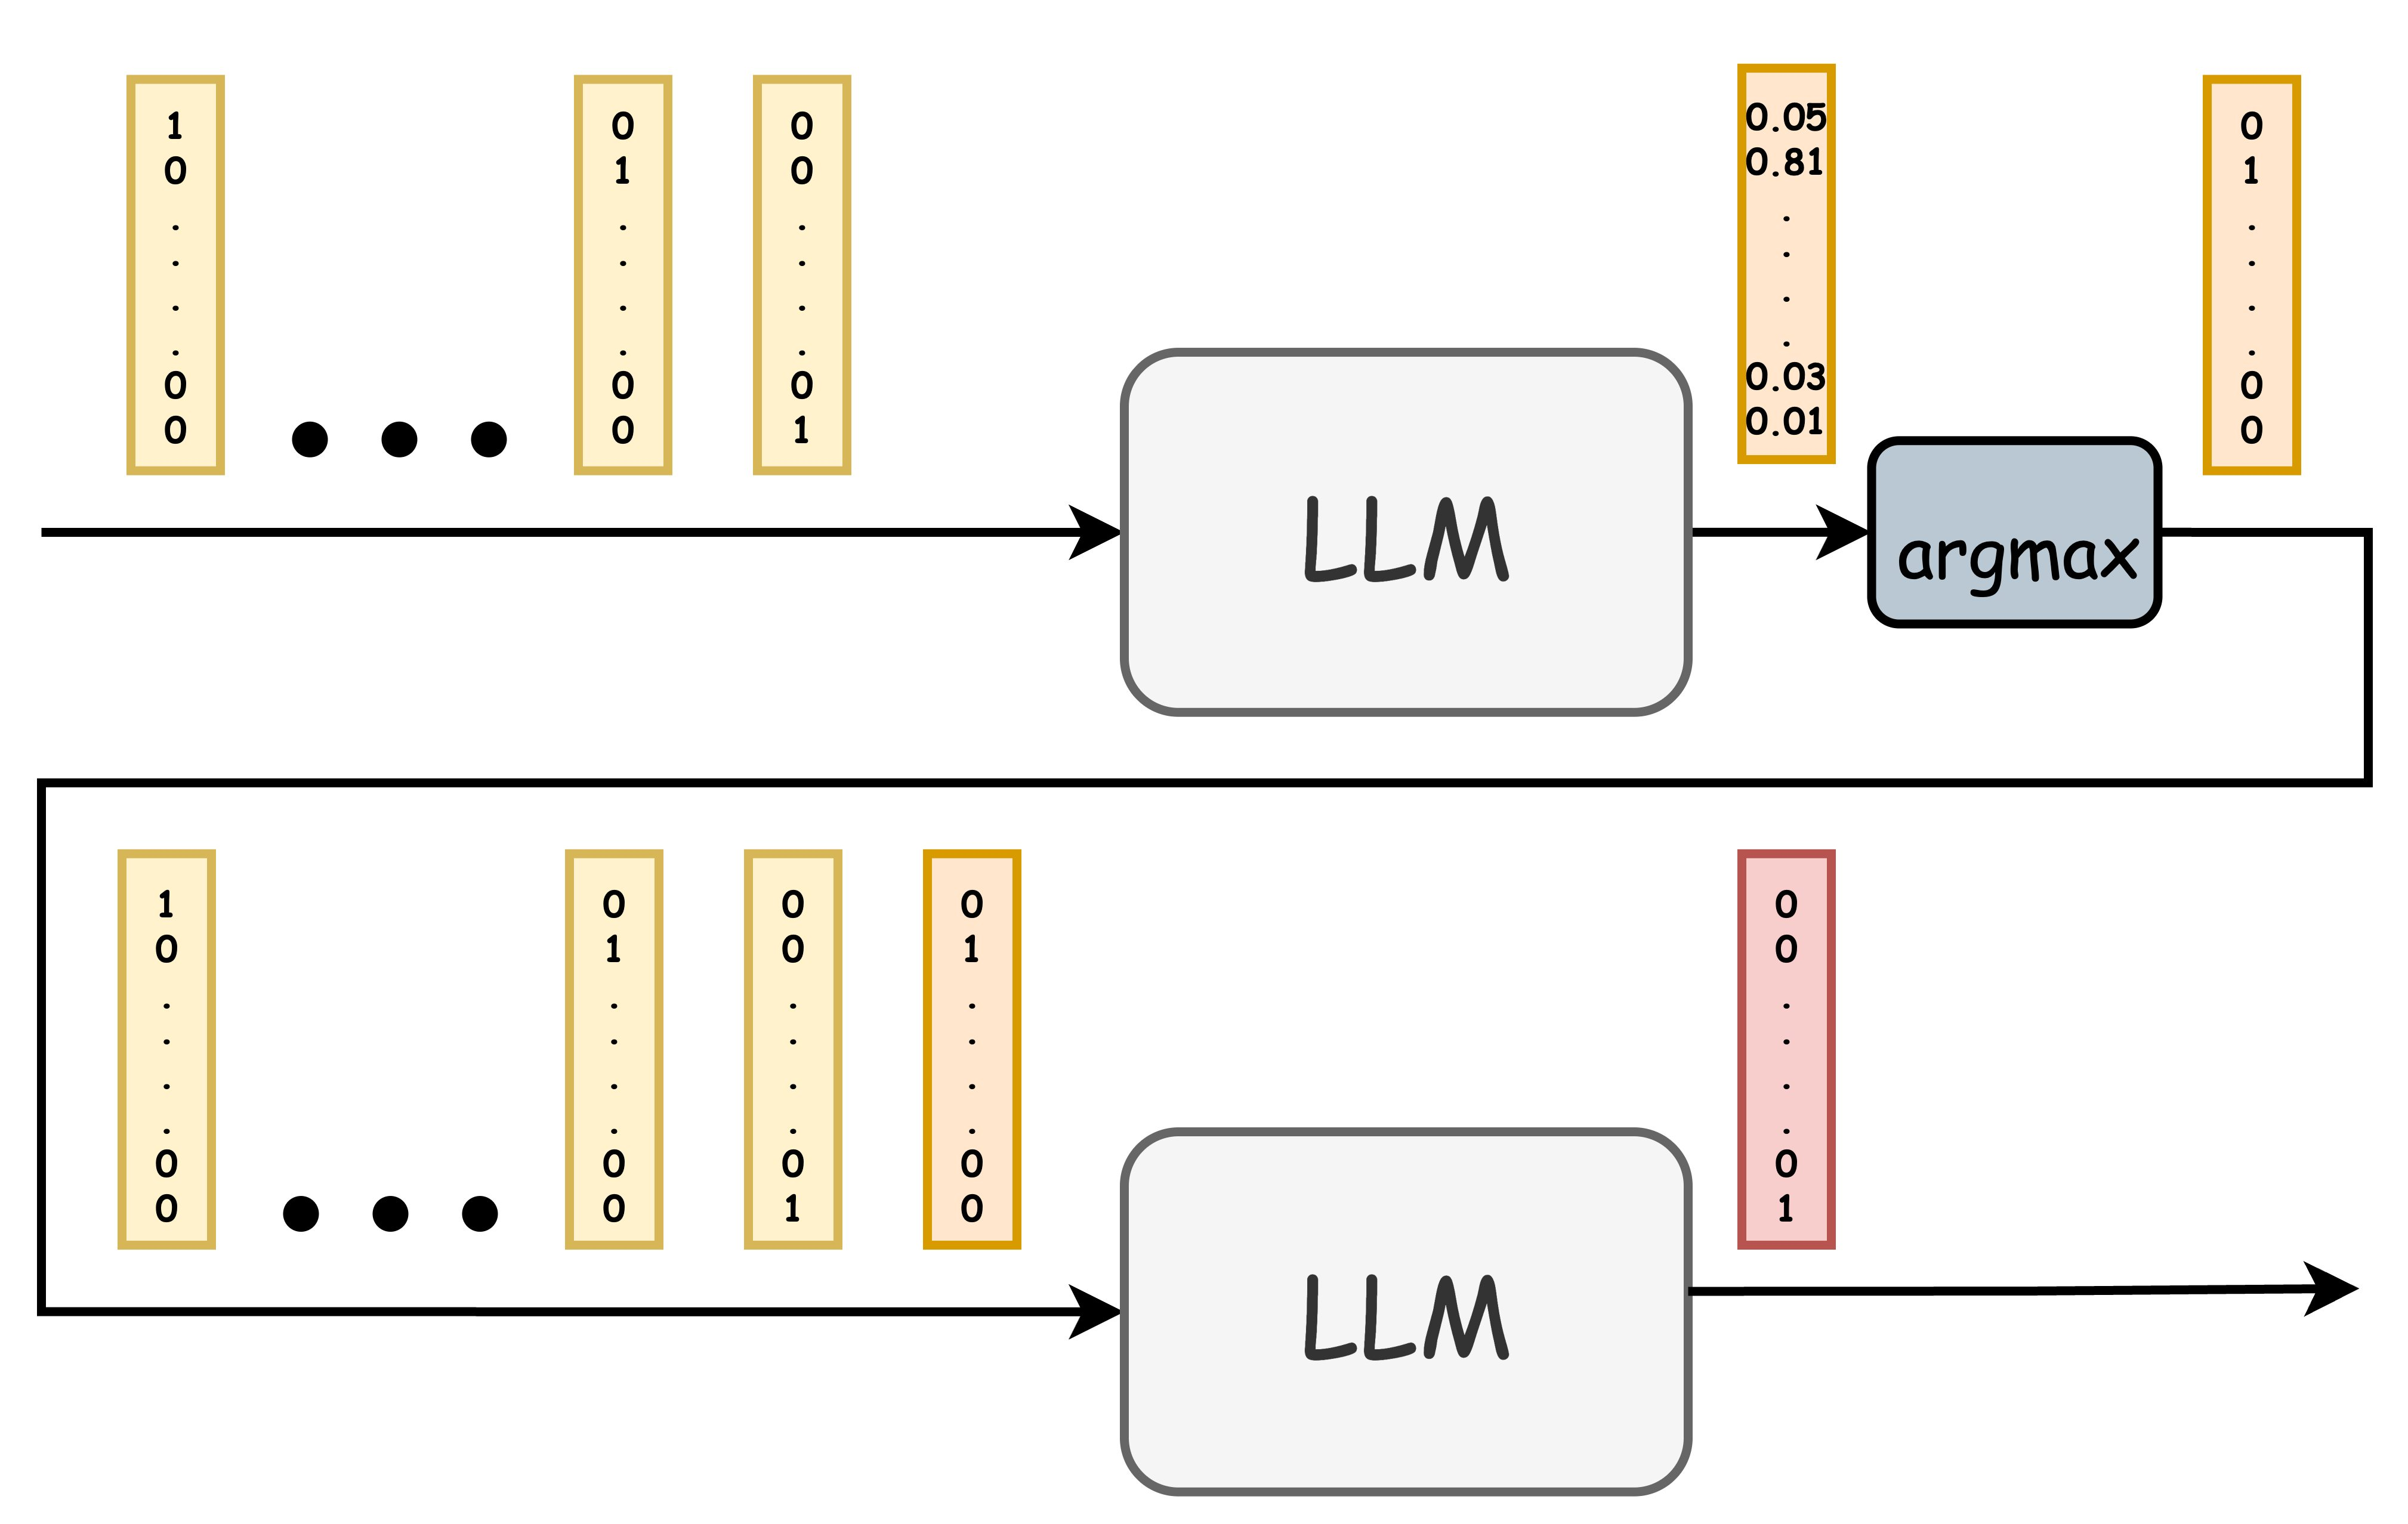
\includegraphics[width=0.5\textwidth]{graphs/ser1.jpeg}
  \caption{Visualization of the "without training" approach, p1}
  \label{fig:ser1}
\end{figure}

\begin{figure}[hbt]
  \centering
  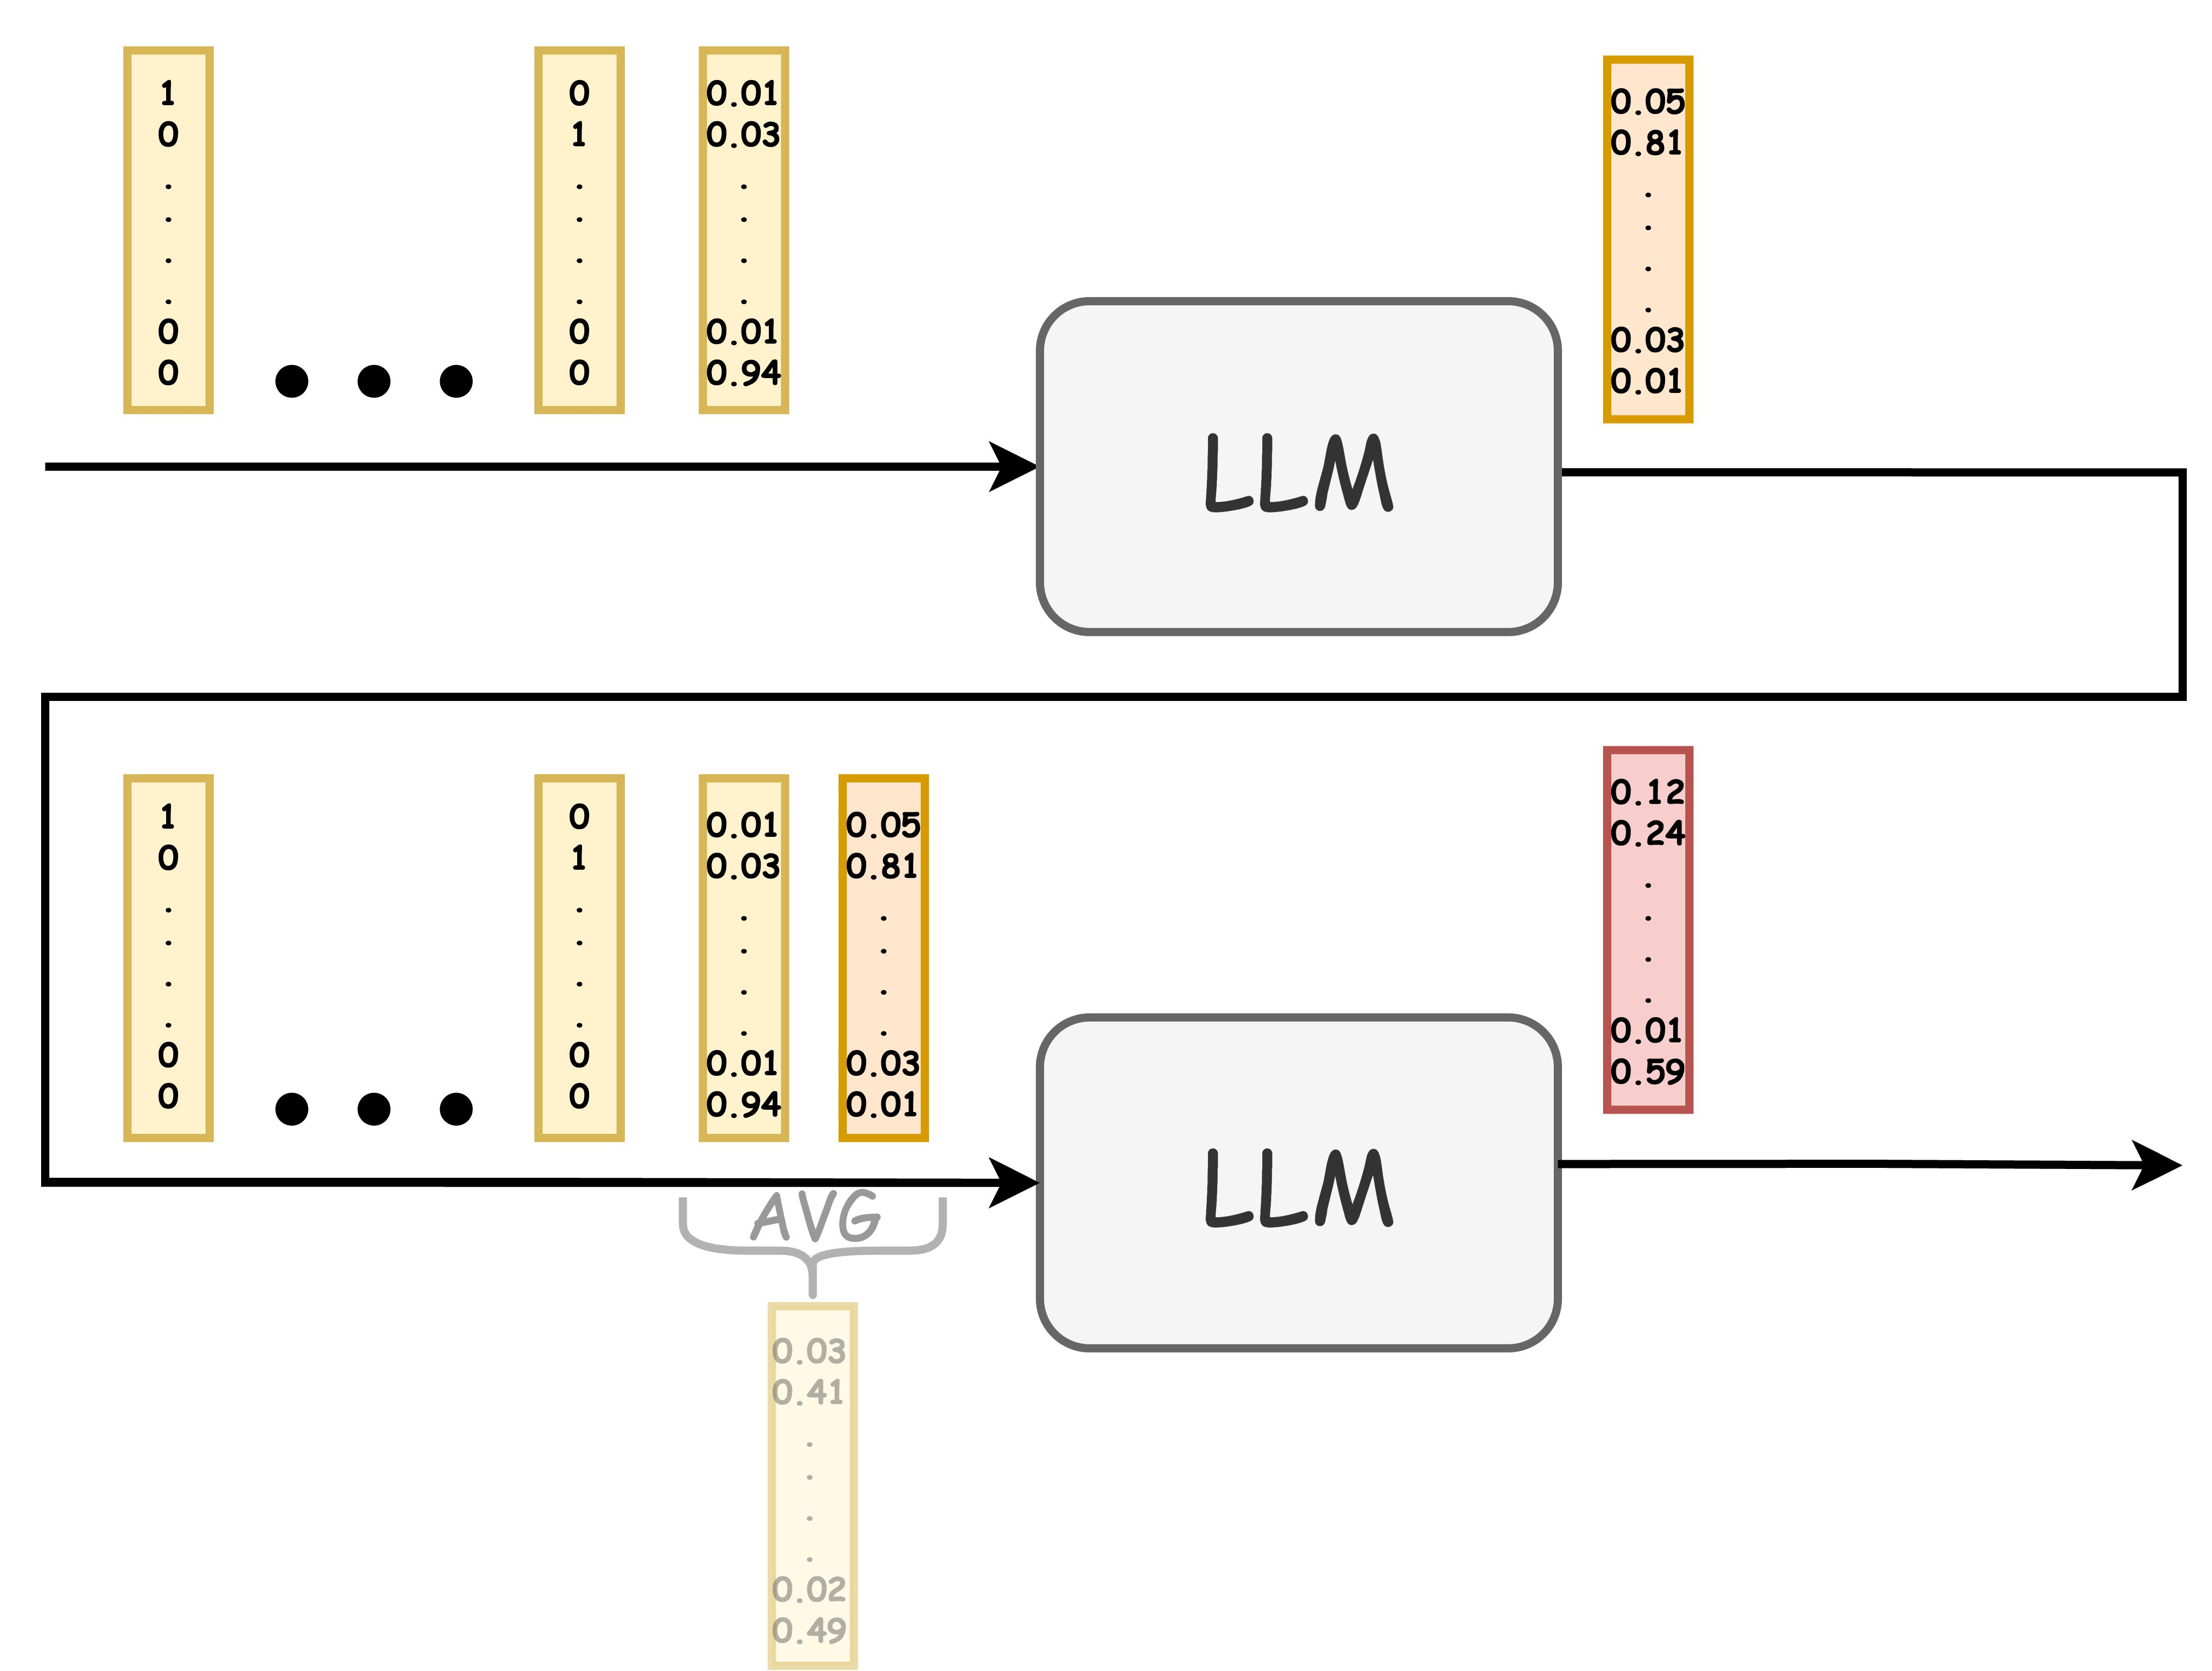
\includegraphics[width=0.3\textwidth]{graphs/ser2.jpeg}
  \caption{Visualization of the "without training" approach, p2}
  \label{fig:ser2}
\end{figure}


\section{Initial Prototype Experiments: First Attempts at Training}

Having established in \S5.1 that naively averaging ("avg, ×2") adjacent embeddings sharply degrades QA quality, we next asked whether a learned projection inserted at the embedding interface could recover performance under the same $2\times$ compression ratio.
The motivation was that, if the embedding manifold is non-linear, a trained projection might learn a geometry-preserving down-map that simple averaging cannot provide.
The baseline (Step 1) and the "soft/hard mix works" observation (Step 2) are illustrated in \ref{fig:steps1-3} and frame this question empirically.

\begin{figure}[hbt]
  \centering
  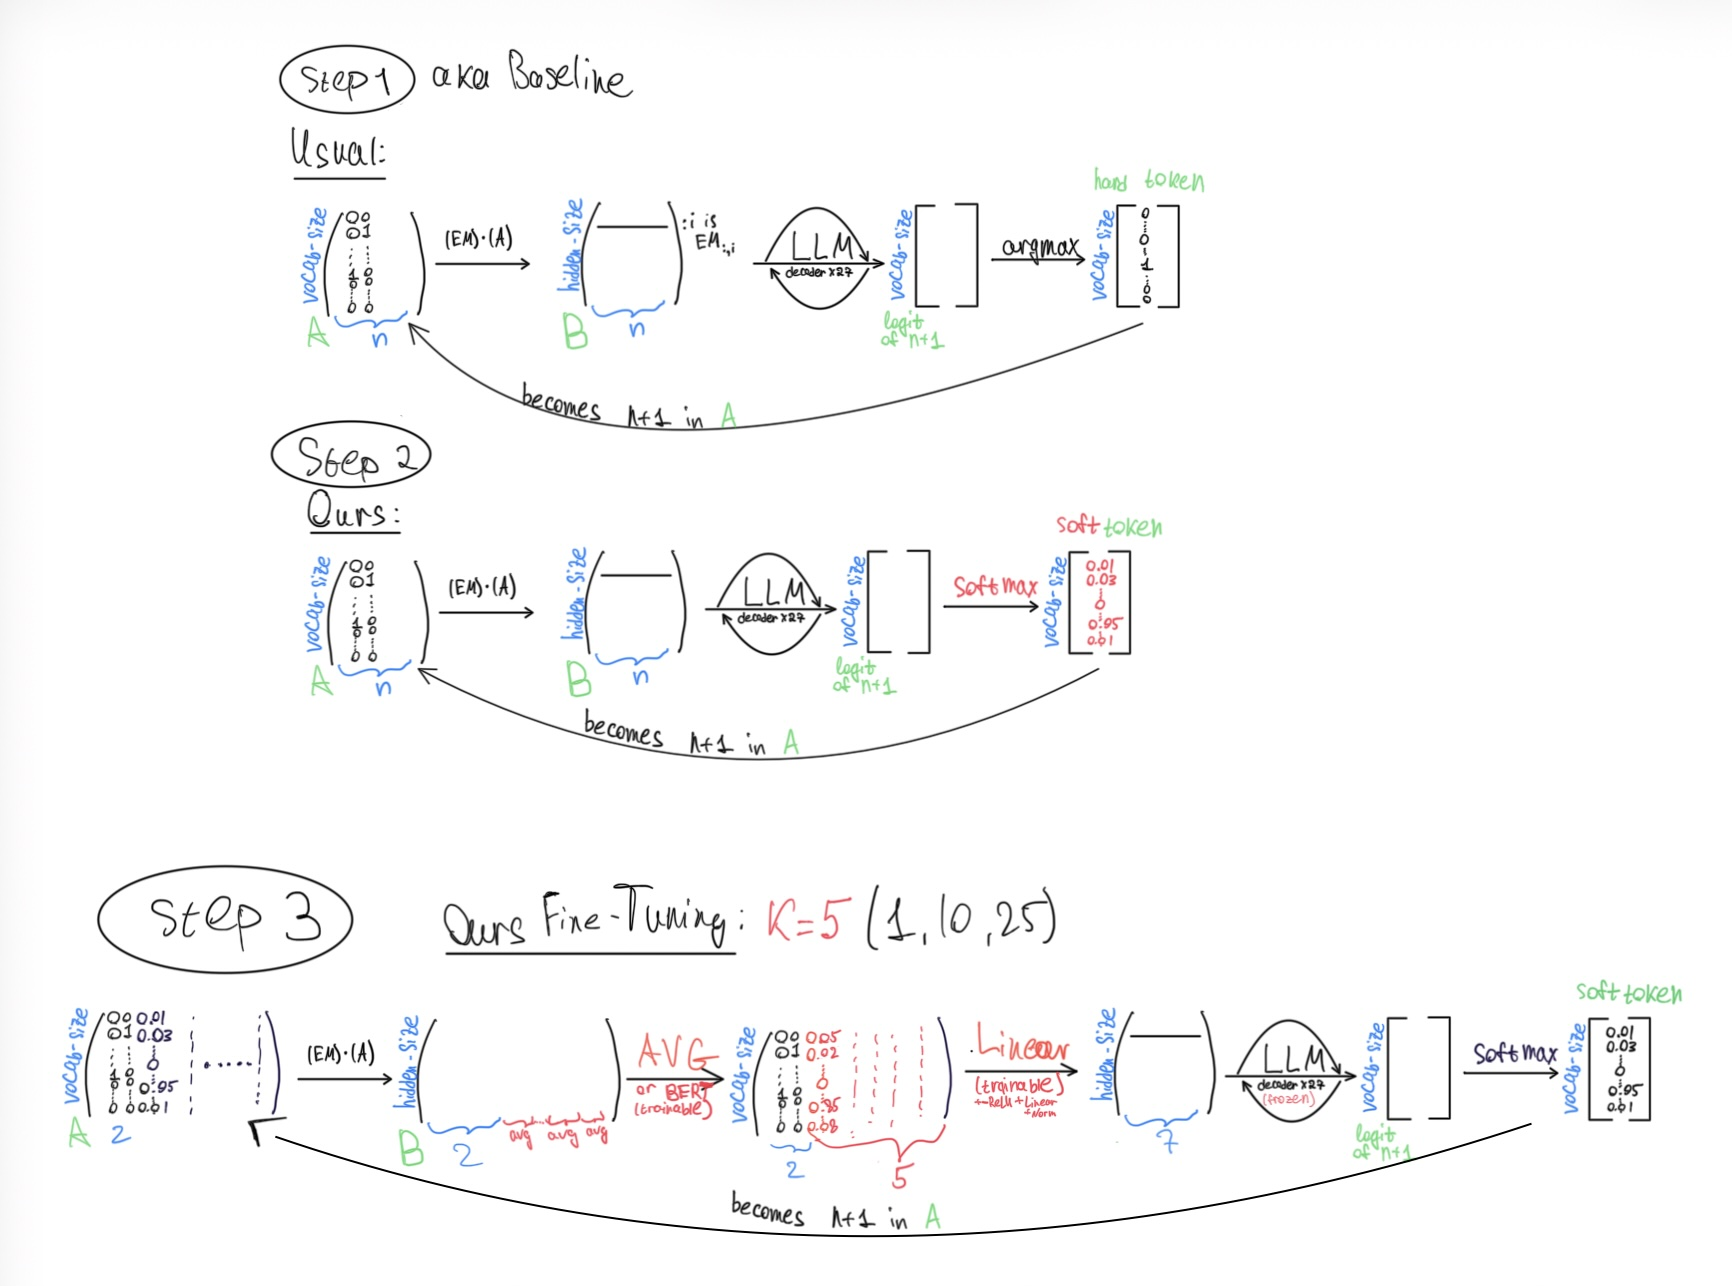
\includegraphics[width=0.5\textwidth]{graphs/steps1-3.jpg}
  \caption{Visualization of the baseline approach, step 1-3; should be redrawn}
  \label{fig:steps1-3}
\end{figure}  

\paragraph{Architectural variants}
We explored minimal-capacity projections that compress two adjacent hidden vectors into one "soft token" acceptable to the frozen decoder.
The first family was a \textbf{linear projector}, $g_\theta:\mathbb{R}^{2d}\to\mathbb{R}^{d}$, applied to $[e_{2t-1};e_{2t}]$ with optional residual gating on the arithmetic mean to stabilize scale.
The second family was a shallow non-linear MLP (one--two layers with GELU), again mapping $2d\to d$.
A third variant inserted a full BERT encoder \cite{devlin2018bert} (12 layers, 768-dimensional hidden states) to process the concatenated embeddings $[e_{2t-1};e_{2t}]$ and produce a single compressed representation, which was then projected back to the decoder's dimensionality.
This encoder-based approach provided substantially higher capacity than the shallow projections, allowing the model to learn more complex compression patterns through its multi-layer self-attention mechanism.
These designs follow the "trainable averaging" schematics shown on \ref{fig:step35}.

\begin{figure}[hbt]
  \centering
  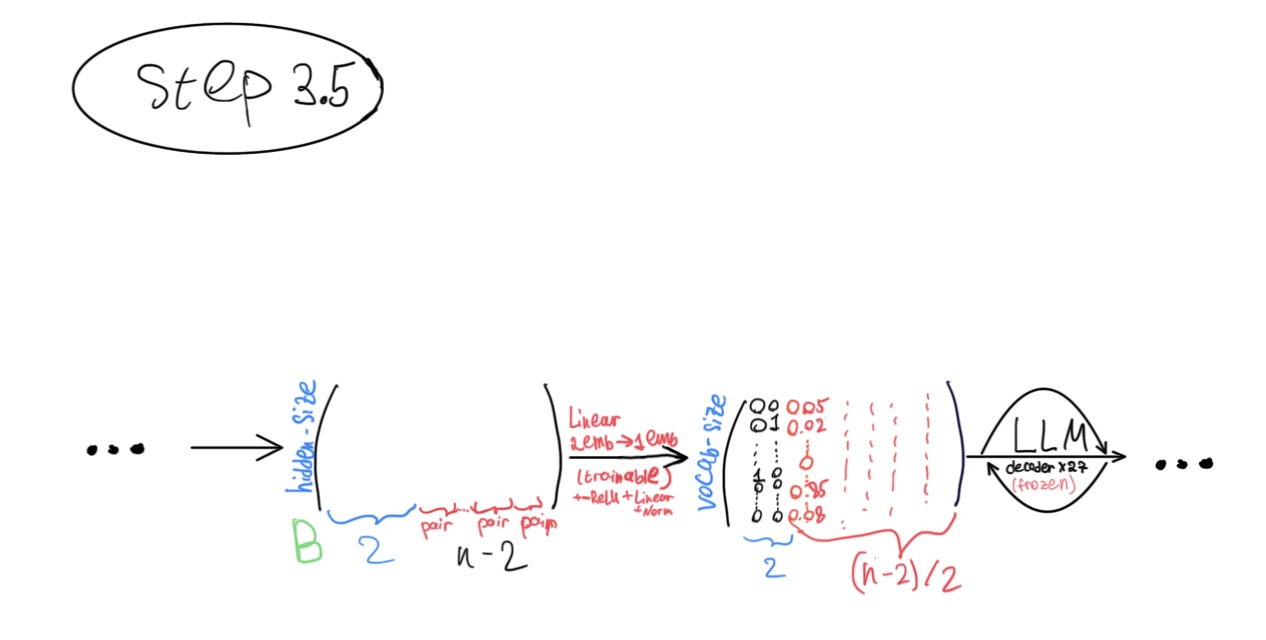
\includegraphics[width=0.5\textwidth]{graphs/step3.5.jpg}
  \caption{Visualization of the experimental setup, step 3.5; should be redrawn}
  \label{fig:step35}
\end{figure}  

\paragraph{Training protocol and results}
All experiments used the SQuAD \cite{squad} "context-embed" setting from \S5.1, keeping Qwen3-8B frozen and training only the projection parameters via token-level cross-entropy on answer continuations.
After verifying the pipeline on a single batch, we trained on SQuAD train and evaluated on validation.
Across linear, MLP, and BERT projections, models quickly overfit but did not generalize: validation loss flattened after early improvement (\ref{fig:losses_squad_1}), and EM/F1 remained well below the hard-token baseline, never closing the large gap to the no-compression control (e.g., the $\sim 50\%$--$80\%$ relative F1 drop visible for averaging).

\begin{figure}[hbt]
  \centering
  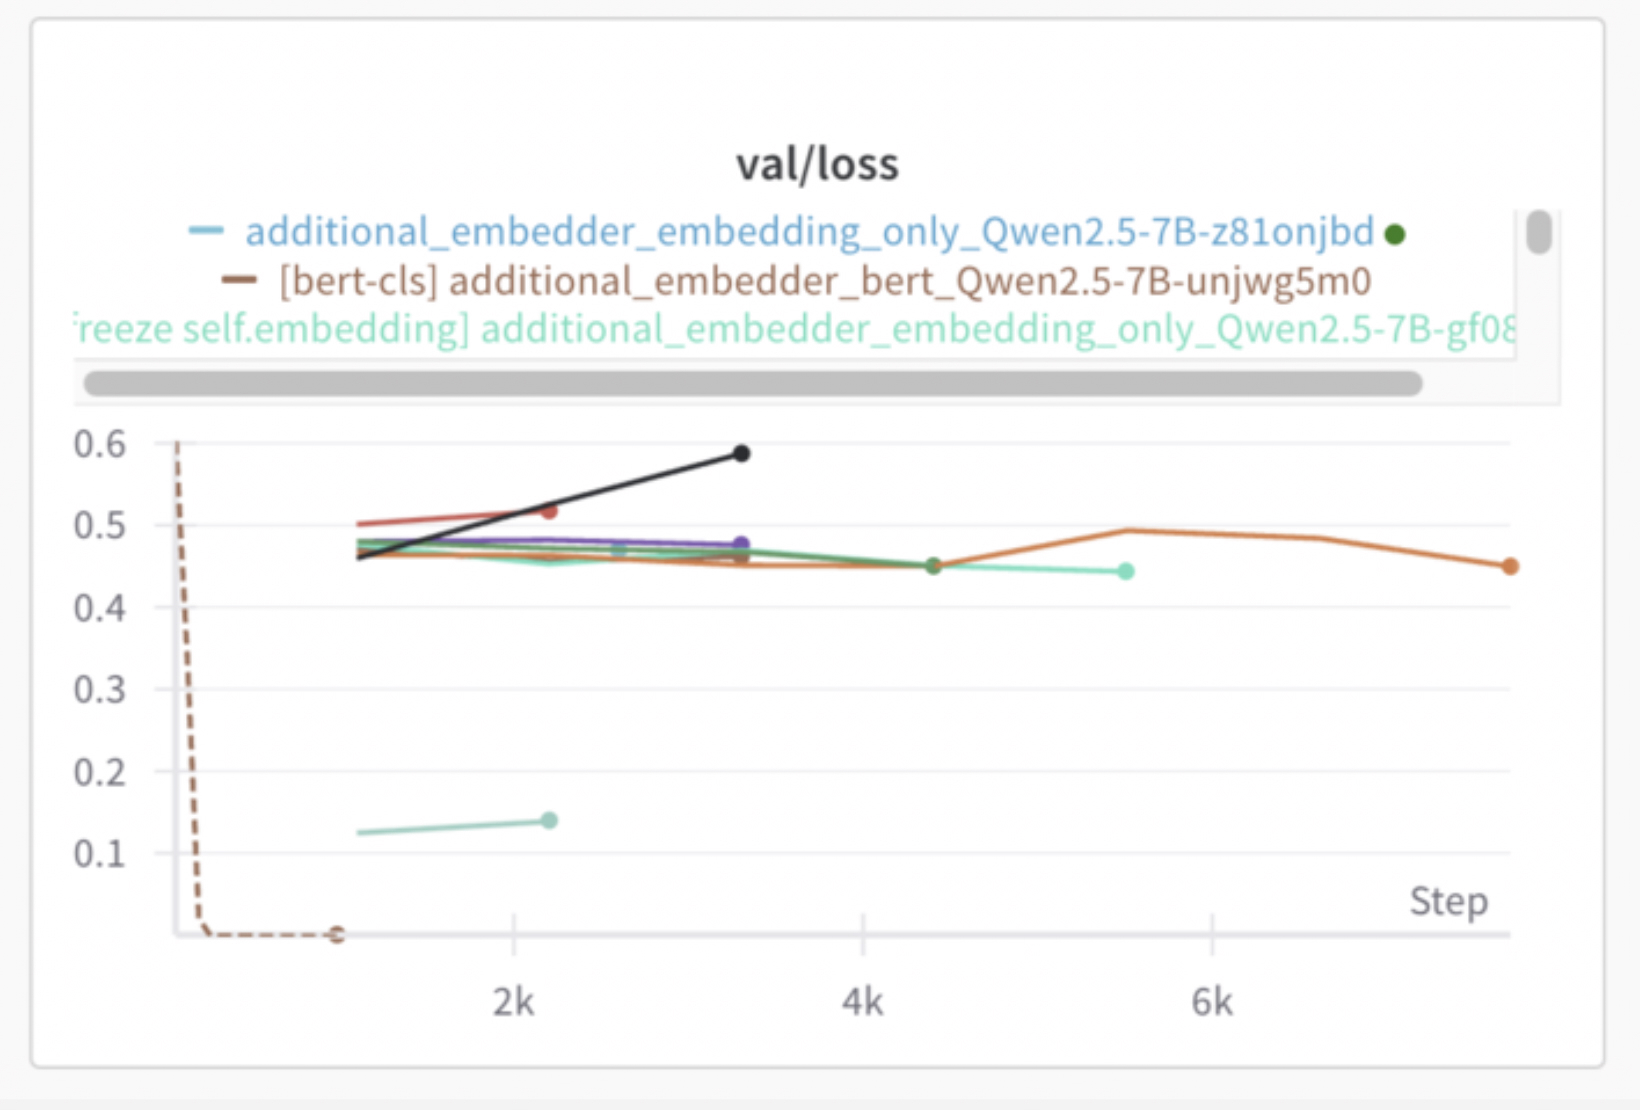
\includegraphics[width=0.5\textwidth]{graphs/losses_squad_1.jpg}
  \caption{Validation loss curves for the SQuAD generalization experiment using linear, MLP and BERT}
  \label{fig:losses_squad_1}
\end{figure}  


\paragraph{Ablation studies}
We varied:
\begin{itemize}
    \item projection type (linear vs.\ 1- or 2-layer MLP),
    \item normalization (pre/post LayerNorm, scale-preserving residual gates),
    \item regularization (weight decay, dropout), and
    \item the decision to re-project via vocabulary space versus staying in hidden space.
\end{itemize}
We also tried unfreezing the token embedding table while keeping the transformer blocks frozen.
None of these changes altered the qualitative outcome: projections still overfit quickly and failed to surpass the baseline (\ref{fig:steps1-3}) in EM/F1.
These negative findings echo the summary on the checkpoint deck ("all our fine-tuning techniques do not recover quality").

\paragraph{Hypotheses for the failure}
Two factors appear decisive.

Firstly, we hypothesize that if the embedding manifold is not smooth, merging two embeddings into one may lose critical geometric structure that the frozen decoder relies on, making it impossible for a simple projection to preserve the information needed for downstream tasks.


Secondly, we hypothesize that the fundamental limitation is the expressive power of the overall model architecture.
Even though the BERT encoder contains 0.1B parameters (more than the projections), it lacks the capacity to learn effective compression when paired with a frozen 8B decoder.

This observation motivated our transition to the ICAE framework, where training LoRA adapters ($\approx$2\% of the 8B model's weights) provides substantially greater expressive power by modulating the decoder's internal representations, despite involving fewer trainable parameters than the full BERT encoder.


\paragraph{Summary}
The experiments illustrated in \ref{fig:step35} demonstrate that trainable projections are insufficient to recover QA performance under $\approx2\times$ compression.
These results motivated us to explore larger-scale training approaches and alternative solutions such as the ICAE framework.


%Pretrained ICAE \cite{ge_-context_2024} demonstrated the ability to decompress general texts almost perfectly.
%High BLEU scores were achieved on datasets like PWC (99.1 for Mistral-7B, 99.5 for Llama-2-7B) and SQuAD (98.1 for Qwen3-8B), indicating that memory slots retained almost all context information for contexts up to 400 tokens.
%Analysis of reconstruction errors showed patterns similar to human memorization mistakes (e.g., restoring "large pretrained language model" as "large pretrained model"), suggesting the model selectively emphasizes or neglects information based on its understanding.

\section{ICAE Pretraining and Evaluation on General Text Reconstruction}

We evaluate ICAE autoencoding (AE) pretraining using Qwen3-8B as the base model.
During AE, the encoder compresses input contexts at a fixed $\times 4$ ratio (specifically, $1024\!\to\!256$ tokens on average), and the decoder reconstructs the original text.
We report BLEU on SQuAD contexts tested on 100 samples.
The checkpoint \texttt{pretrain\_2607\_1024\_4\_1B/checkpoint-12000} is selected as the main run and used for fine-tuning.

\begin{table}[h]
    \centering
    \small
    \setlength{\tabcolsep}{6pt}
    \begin{tabular}{lll c}
        \toprule
        \textbf{Run} & \textbf{Checkpoint (\# steps)} & \textbf{Compression} & \textbf{BLEU (mean, n=100)} \\
        \midrule
        Qwen3-8B/full (no ICAE) & 18k & $\times 1$ & 0.867 \\
        \addlinespace
        ICAE PT (pretrain\_1207) & 9k & $\times 4$ & 0.942 \\
        ICAE PT (pretrain\_1207) & 12k & $\times 4$ & \textbf{0.964} \\
        ICAE PT (pretrain\_1207) & 27k & $\times 4$ & 0.902 \\
        \addlinespace
        ICAE PT (pretrain\_2607\_1024\_4\_1B) & 9k  & $\times 4$ & 0.909 \\
        ICAE PT (pretrain\_2607\_1024\_4\_1B) & 12k (main) & $\times 4$ & \underline{0.936} \\
        ICAE PT (pretrain\_2607\_1024\_4\_1B) & 18k & $\times 4$ & 0.928 \\
        \bottomrule
    \end{tabular}
    \caption{Autoencoding (AE) reconstruction BLEU on SQuAD contexts (100-sample evaluations only). The \texttt{pretrain\_2607\_1024\_4\_1B} 12k checkpoint is the main model used for FT.}
    \label{tab:ae_bleu_squad_ours}
\end{table}

\medskip
We have also experimented with compressing 16 tokens into 4 on average instead of 1024 into 256.
It which achieved a higher BLEU (\(\approx 0.982\)). 
Notably, none of the 100-sample AE scores reach \(\approx 0.99\).
This may be acceptable for general text but could be material for code, where near-lossless reconstruction is likely a prerequisite for downstream stability.

\medskip
\noindent\textit{Example} 
Below we show a short example, where we tried to reconstruct the README.md file of the SWE-agent project.
The difference is highlighted in yellow.

\noindent\textbf{Original:}

\quad\texttt{<p align="center">}

\quad\texttt{<a href="https://swe-agent.com/latest/">}

\quad\texttt{<strong>Documentation</strong></a>\&nbsp; ...}

\noindent\textbf{Reconstructed:}

\quad\texttt{<p align="center">}

\quad\texttt{<a href="https://swe-agent.com}\colorbox{yellow}{\texttt{/agent/}}\texttt{latest/">}

\quad\texttt{<strong>Documentation</strong></a>\&nbsp; ...}

\noindent Even in the very start of the text, the difference is noticeable: the hallucinated \texttt{/agent/} path segment in the URL, which could break navigation in a coding task.


In line with internal feedback, these AE findings suggest that the current pretrain/fine-tuning mixes undertrain the model on code: AE BLEU for code should approach text-level (near 1.0) to avoid even small inaccuracies (e.g., link/variable name substitutions).



% ========================================
% SECTION 5.3: EVALUATION ON QUESTION ANSWERING TASKS (OFFLINE)
% ========================================
\section{ICAE Fine-Tuning and Evaluation on Question Answering Tasks}

While the original ICAE work \cite{ge_-context_2024} demonstrated promising results on their proprietary PWC dataset, we sought to validate these findings on a well-established benchmark to ensure generalizability and facilitate fair comparison with existing approaches.
To address the limitation of the authors'-crafter PWC dataset, we conducted fine-tuning experiments on the Stanford Question Answering Dataset (SQuAD) \cite{squad}, a widely recognized benchmark in the question answering literature that provides standardized evaluation protocols and enables reproducible comparisons.

The fine-tuning procedure follows the encoder-decoder structure established during pretraining, with modifications to accommodate the question answering objective.
During fine-tuning, we feed compressed context representations produced by the encoder into the decoder, concatenated with uncompressed question tokens.
The decoder then generates answer from this mixed representation, while throught backpropagation we update the LoRA weights of the encoder.
This setup encourages the encoder to learn compression strategies that preserve information necessary for the decoder to extract answers from.
We employ LoRA fine-tuning \cite{hu2021lora} with identical hyperparameters to those used in the original ICAE pretraining to maintain consistency and enable fair comparison.

To establish a comprehensive evaluation baseline, we compare four distinct model configurations that systematically vary the training procedure and compression strategy.
First, we evaluate the base Mistral-7B model \cite{mistral7b} without any fine-tuning to establish the zero-shot performance ceiling.
Second, we construct a LoRA fine-tuned baseline where we apply LoRA fine-tuning directly to Mistral-7B on the SQuAD dataset without any compression mechanism, thus representing the standard approach without context condensation.
This baseline operates without an encoder-decoder structure, functioning as a conventional LLM fine-tuned for question answering at full context length.
Third, we evaluate the ICAE model fine-tuned on PWC as provided by the original authors \cite{ge_-context_2024}, which represents their reported best configuration.
Finally, we train our own ICAE variant by fine-tuning the pretrained encoder-decoder architecture on SQuAD using identical training code and hyperparameters to those employed by the authors for PWC fine-tuning.
This parallel setup enables direct comparison while controlling for implementation differences.

Table~\ref{tab:icae_squad} presents the evaluation results across all four configurations, measured using Exact Match (EM) and F1 scores on the SQuAD validation set.
The compression ratio for ICAE variants averages approximately $1.7 \pm 0.7$, meaning contexts are condensed to roughly 60\% of their original length while maintaining the compressed representation.
\begin{table}[h]
    \centering
    \begin{tabular}{lccc}
        \toprule
        \textbf{Model} &
        \textbf{Compression} &
        \textbf{Exact Match} &
        \textbf{F1} \\
        \midrule
        Mistral-7B (no FT)          & ×$1$         & 49 & 68 \\
        LoRA-FT baseline            & ×$1$         & \underline{59} & \underline{65} \\
        ICAE FT (PwC, authors)       & ×$1.7\pm0.7$ & 41 & 57 \\
        ICAE FT (SQuAD, ours)              & ×$1.7\pm0.7$ & \textbf{69} & \textbf{73} \\
        \bottomrule
    \end{tabular}
    \caption{ICAE averaging on SQuAD}
    \label{tab:icae_squad}
\end{table}

Several important observations emerge from these results.
First, our ICAE fine-tuning on SQuAD achieves the highest performance across both metrics, with an F1 score of 73 and Exact Match of 69, representing substantial improvements over both the untrained baseline and the LoRA fine-tuned control.
Notably, this performance gain occurs despite operating under approximately 2× compression, suggesting that the learned compression strategy successfully preserves task-critical information while reducing computational overhead.

Most strikingly, the compressed ICAE model not only outperforms the uncompressed baseline (already valuable given the computational savings) but also surpasses the uncompressed LoRA fine-tuned baseline by 8 F1 points (73 versus 65).
This result is quite unexpected: compression typically implies information loss, yet here the compressed model demonstrates superior performance to its uncompressed counterpart trained with identical LoRA fine-tuning procedures.
We hypothesize that this advantage stems from the compression mechanism's ability to filter and retain only the most importnat information from the context, effectively introducing a beneficial inductive bias.
This might help the model focus on task-relevant features while discarding noise or redundant details.

Moreover, the ICAE model fine-tuned on PWC exhibits notably lower performance than all other configurations, achieving F1 and EM scores of 57 and 41 respectively.
This result indicates that the PWC-fine-tuned model fails to generalize effectively to the SQuAD evaluation distribution, despite achieving strong performance on its training domain.
This performance gap suggests potential overfitting to the specific characteristics of the PWC dataset, which may have properties that do not transfer well to standard question answering benchmarks.

These results provide encouraging evidence for the viability of applying ICAE-based compression to downstream tasks beyond the original evaluation domain.
The strong performance on SQuAD, combined with the observed compression benefits, motivated our subsequent investigation of the ICAE framework in more complex, agentic settings where context length presents significant computational challenges.

\section{[Very main part?] ICAE Fine-Tuning and Evaluation on SWE-bench Verified}

Here we describe the main experiment of the thesis and discuss its results.
We should start by describing the pictures \ref{fig:mega1} and \ref{fig:mega2}.
Picture \ref{fig:mega1} discribes our contribution - training procedure of ICAE model to an agentic scenario (more specifically SWE-bench Verified dataset).
Firstly, we have trajectories to train on (generated by Claude and described in Section~\ref{sec:4.1.3}).
Then, we explain how to train useing them.
One reajectory is basically a loop of LLM making Step K (this generates tool call), then we provide it to the environment and recieve an observation. 
Observation is then passed to LLM's step K+1, and so on.
In the strart there is an uncompressed user prompt.
Compression happens for every observation, so that the decoder Qwen3 never sees any observation longer than 256 tokens in plain text, only in compressed form (embeddings).


More details of the LLM's step are in the picture \ref{fig:mega2}. It is one LLM's step in detail.
The observation is passed to encoder, which produces compressed representation of the observation.
Then this compressed representation (with all the previous history obviously) is passed to the decoder, which generates the next tool call for the next step.
We then compute the loss as a cross-entropy on the tool call token-by-token, since we have the reference tool call from smarter model; and backpropagate through the decoder and the encoder (only LoRA weights of the encoder are updated).
Note that the encoder and decoder models are both qwen3 and same. 
The only difference is that the encoder has a LoRA adapter, which is trained to produce compressed representations of the observations.

\begin{figure}[hbt]
  \centering
  
\includegraphics[width=0.8\textwidth]{graphs/mega-1.jpeg}
  \caption{ICAE application to SWE-bench}
  \label{fig:mega1}
\end{figure}

\begin{figure}[hbt]
  \centering
  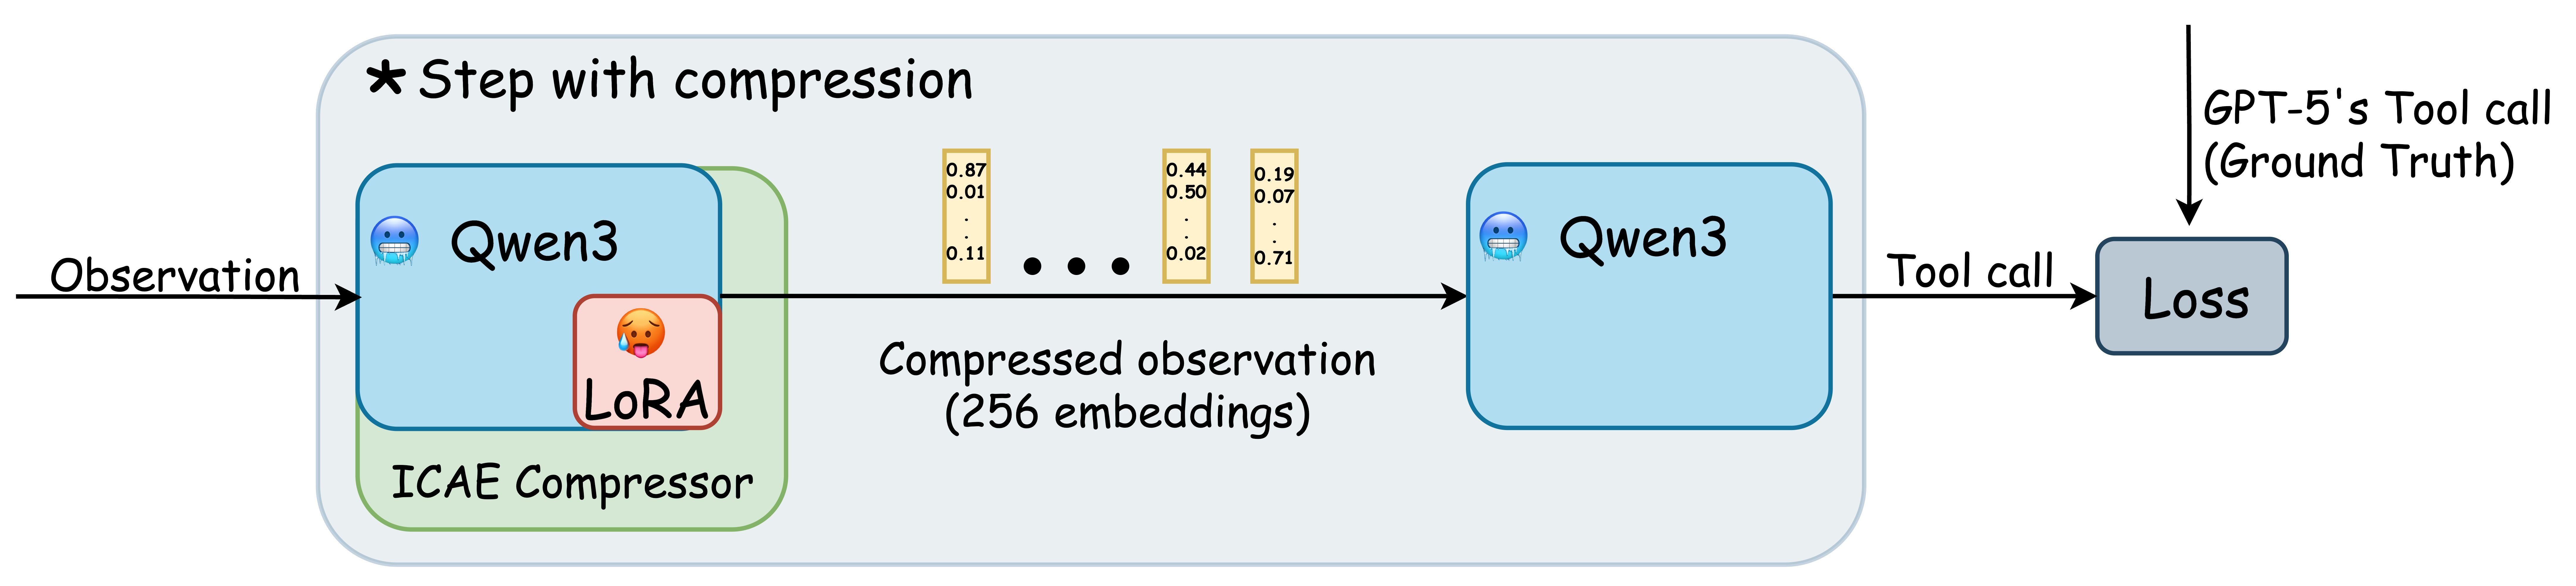
\includegraphics[width=0.8\textwidth]{graphs/mega-2.jpeg}
  \caption{ICAE application to SWE-bench}
  \label{fig:mega2}
\end{figure}

Then we have to describe the results in the table \ref{tab:qwen_icae_variants_absolute}.
First of all we need to describe the table structure: we have 5 columns: Encoder, Decoder, Accuracy, Time and Resolved.

Encoder is the model that is used to compress the observations ("---" means no encoder).

Decoder is the model that is used to generate the next tool call ("Qwen" means uncompressed Qwen3-8B, "Qwen-LoRA-FT" means LoRA fine-tuned Qwen3-8B, "Qwen-Full-FT" means full fine-tuned Qwen3-8B).

Accuracy is the token-wise accuracy of the model on the SWE-bench Verified dataset (described in more details in Section~\ref{sec:4.4})

Resolved is the number of issues resolved by the model (resolved issues / total issues) out of 500 issues.

Time is the time taken by the model to generate the next tool call (mean time per tool call) in seconds.

Then we have to describe the results in the table.


%\begin{table}[h]
%    \centering
%    \setlength{\tabcolsep}{6pt}
%    \begin{tabular}{llcc}
%        \toprule
%        \textbf{Encoder} & \textbf{Decoder} & \textbf{Accuracy} & \textbf{Mean tool-call time (s)} \\
%        \midrule
%        % --- Baseline encoder
%        —                        & Full-FT   & 0.9484 & 1.24 \\
%        —                        & LoRA-FT   & 0.9118 & 1.24 \\
%        —                        & Qwen           & 0.8967 & 1.23 \\
%        \addlinespace
%        % --- Ablations
%        del long obs-s             & Qwen           & 0.8873 & 0.44 \\
%        del all obs-s              & Qwen           & 0.8802 & 0.39 \\
%        \addlinespace
%        % --- ICAE (Qwen pretrained) encoder
%        ICAE (LoRA-PT w/ Full-FT)   & Full-FT   &  0.9219    &  — \\
%        ICAE (LoRA-PT w/ Qwen)    & Qwen           &  0.8808 & \textbf{1.12 (0.31+0.81)} \\
%        \addlinespace
%        % --- ICAE (Qwen-LoRA-FT) encoder
%        ICAE (LoRA-FT)         & Full-FT   &  ?   & —  \\
%        ICAE (LoRA-FT)         & LoRA-FT   & 0.9263   & —  \\
%        ICAE (LoRA-FT)         & Qwen           & 0.9020 & — \\
%        % bad-seed ICAE (LoRA-FT)         & Qwen           & 0.8918 & — \\       
%
%        
%        \bottomrule
%    \end{tabular}
%    \caption{No think bug table. Qwen and ICAE future variants. FT=FineTuning, PT=PreTraining}
%    \label{tab:icae_variants}
% \end{table}

\begin{table}[h]
  \centering
  \small
  \setlength{\tabcolsep}{4pt}

  \begin{tabular}{|ll|ccc|}
      \hline
      \textbf{Encoder} & \textbf{Decoder} & \textbf{Acc. $\uparrow$} & \textbf{Resolved (/500) $\uparrow$} & \textbf{Time (s) $\downarrow$} \\
      \hline
      \multicolumn{5}{|l|}{\hspace{1em}\textit{Naive Baselines}} \\
      \hline
      del long obs-s            & Qwen           & 0.8873 & 1         & 0.44                      \\
      del all obs-s             & Qwen           & 0.8802 & 0         & 0.39                      \\
      \hline
      \multicolumn{5}{|l|}{\hspace{1em}\textit{Baselines}} \\
      \hline
      —                         & Qwen-Full-FT   & \textbf{0.9484} & ??? (waiting for Igor)         & 1.24                      \\
      —                         & Qwen-LoRA-FT   & 0.9118 & 10 (waiting for Igor)        & 1.24                      \\
      —                         & Qwen           & 0.8967 & \textbf{26}        & 1.23                      \\
      \hline
      \multicolumn{5}{|l|}{\hspace{1em}\textit{ICAE-FT Compression}} \\
      \hline
      ICAE (Qwen-LoRA-FT)       & Qwen           & 0.9020 & \underline{11}        & \textbf{1.12 (0.31+0.81)}    \\
      ICAE (Qwen-LoRA-FT)       & Qwen-LoRA-FT   & \underline{0.9263} & 3 (overfit?) & 1.13                      \\
      \hline
      \multicolumn{5}{|l|}{\hspace{1em}\textit{ICAE-PT Compression (Ablation)}} \\
      \hline
      ICAE (Qwen-LoRA-PT w/ Q-Full-FT) & Qwen-Full-FT   & 0.9219 & —         & —                         \\
      ICAE (Qwen-LoRA-PT w/ Qwen)      & Qwen           & 0.8808 & —         & -        \\
      \hline
  \end{tabular}
  \caption{No think bug table. Qwen and ICAE future variants. FT=FineTuning, PT=PreTraining}
  \label{tab:qwen_icae_variants_absolute}
\end{table}


Efficiency Results: ICAE \cite{ge_-context_2024} compression led to measurable efficiency improvements, achieving a theoretically 10\% faster mean tool-call generation time than the vanilla baseline (e.g., 0.4880s vs 0.5437s).
Furthermore, latency tests showed speedups of 2.2× to 3.6× in total time for inference.
Token-wise Accuracy vs. Resolved Rate: Although token-wise accuracy performed on par with (or slightly better than) the vanilla Qwen baseline (e.g., 0.9089 vs 0.9000), this metric was noted to be problematic ("token-wise accuracy is bullshit") and decoupled from true task success.
End-to-End Task Success: The primary negative finding was that the model with compression resolved significantly fewer than 50\% as many issues as the original Qwen model on the SWE-bench Verified dataset.


% ========================================
% SECTION 5.x: DISABLING THINKING EXPERIMENTS
% ========================================
\section{Disabling Thinking Experiments}
\label{sec:disabling_thinking}

\textbf{TODO: maybe we push it to appendix?}

We evaluated the impact of disabling thinking by inserting the token sequence \texttt{\textbackslash think \textbackslash think} with a newline marker during decoding.
We tested two variants: adding the sequence after every step and adding it only once at the end.
Surprisingly, the approach commonly suggested by authors (frequent insertion) yielded worse output quality than the minimal, end-only variant in our setting.
We note that related observations of atypical Qwen3 behavior under prompting heuristics have been reported anecdotally; a systematic investigation is out of scope for this work. (as a result e.g. coder-30bA3 has no thinking mode at all)
Further details and ablations are left for future work.

\textbf{TODO: maybe add an exmple of this?}
